\documentclass[letterpaper, 12pt]{article}
\usepackage{tabularx} 
\usepackage{amsmath} 
\usepackage{graphicx} 
\usepackage{caption}
\captionsetup[figure]{font=footnotesize}
\usepackage[margin=1.1in,letterpaper]{geometry}
\usepackage{cite} 
\usepackage{textcomp}
\usepackage[final]{hyperref} 
\hypersetup{
	colorlinks=true,      
	linkcolor=blue,        
	citecolor=blue,        
	filecolor=magenta,     
	urlcolor=blue         
}
\usepackage{blindtext}
\usepackage[utf8]{inputenc}
\usepackage[english]{babel}

\usepackage{amsfonts}
\usepackage{amssymb}
%\usepackage{hyperref}


\begin{document}
	
	\title{CMLS Homework 2 - Distortion Effect Plugin}
	\author{Group 11: E. Castelli, E. Intagliata, A. Rizzitiello, G. Zanocco}
	\date{May 2021}
	\maketitle
	
	
	The aim of our project was to develop a distortion plugin using the JUCE framework \cite{juce}.
	Distortion is a non-linear effect used to alter the harmonic content of a sound or an instrument, usually by increasing their gain, producing a "dirty" tone.
	
	Distortion effects can create a wide palette of sounds ranging from smooth, singing
	tones with long sustain to harsh, grungy effects.
	
	In our plugin we decided to implement five kinds of distortion: Hard Clipping, Quadratic Soft Clipping, Exponential Soft Clipping, Full Wave Rectifier, Half Wave Rectifier.
	Each one has a different characteristic curve therefore a different sound timbre.
	
	\section{A bit of theory}
	Distortion of an audio is a \textit{non-linear} effect. This leads to the introduction of new harmonics by memoryless non-linearities.
	
	Distortion effects can be described by its characteristic function. It mathematically maps the input samples directly to the output ones.
	
	The simplest kind of distortion is \textbf{clipping}.
	In the analogue world clipping is achieved pushing an amplifier to create a signal with more power than its power supply can produce. It will amplify the signal only up to its maximum capacity, at which point the signal can be amplified no further. 
	As the signal simply "cuts" or "clips" at the maximum capacity of the amplifier, the signal is said to be "clipping". The extra signal which is beyond the capability of the amplifier is simply cut off, resulting in a sine wave becoming a distorted square-wave-type waveform \cite{clipping}. 
	
	Distortion effects are often classified by whether they produce \textbf{hard clipping} or \textbf{soft clipping}. 
	
	\subsection*{Hard Clipping}
	
	
	Hard clipping limits peaks abruptly, resulting in an increase in higher harmonics. As clipping increases, a tone input progressively begins to resemble a square wave which has odd number harmonics. This produces sharp corners in the waveform and is generally described as sounding "harsh" \cite{distortion}. 
	
	We implemented hard-clipping with characteristic function:
	\begin{equation}
		y(x) =     
		\begin{cases}
			-1 & \text{if $ Gx \leq -1 $,}\\
			Gx & \text{if $ -1 < Gx < +1 $,}\\
			+1 & \text{if $ Gx \geq +1 $,}\\
		\end{cases}       
	\end{equation}
	
	where $G$ is the input gain that can be modified by the users.
	
	\subsection*{Soft clipping}
	
	Soft clipping is characterized by a smooth approach to the clipping level, creating rounded corners at the peaks of the waveform. We have two options for soft clipping. They reflect two implementations which differ in their characteristic function.
	
	The first implementation is called \textbf{quadratic soft-clipping} and its characteristic function is indeed a quadratic function: 
	
	\begin{equation}
		y(x) =     
		\begin{cases}
			2x & \text{if $ 0 \leq |x| < 1/3 $,}\\
			1 -(2-3x)^2 / 3& \text{if $ 1/3 \leq |x| < 2/3 $,}\\
			1 & \text{if $ 2/3 \leq |x| \leq 1 $,}\\
		\end{cases}       
	\end{equation}
	
	In this example, for input samples with magnitude less than 1/3, the
	effect operates in a linear region, but as the magnitude of x increases, it becomes progressively more nonlinear until clipping occurs above $|x| = 2/3$ and the output no longer grows in magnitude. 
	
	The second implementation is the so called \textbf{exponenetial soft-clipping} because its characteristic function is an exponential function:
	
	\begin{equation}
		y(x) = sign(x) ( 1 - e^{-|Gx|} )
	\end{equation}
	
	In this equation, the output asymptotically approaches the clipping point the input gets larger.
	
	The two previous situations are also referred as \textit{overdrive} since there are both regions of linearity and non-linearity.
	
	Overdrive is more pleasant to the listener and it resembles the soft limiting of valves.
	
	
	\subsection*{Rectifiers}
	In the other two implementations distortion is achieved through \textit{rectification}. In rectification the characteristic function is an asymmetrical function.
	
	In \textbf{half-wave rectification} a function that sets the negative half-wave to 0 is used:
	
	\begin{equation}
		y(x) = max(x,0)
	\end{equation}
	
	In \textit{full-wave rectification} the absolute value function is used:
	\begin{equation}
		y(x) = |x|
	\end{equation}
	It simply inverts the negative half-wave. As a result it adds a  strong octave harmonic to the output signal.
	
	Rectification is a strongly non-linear effect , thus it produces a very harsh sound. 
	
	\subsection*{Oversampling and anti-aliasing}
	
	As we said in the beginning of this report, distortion introduces high frequency harmonics which are integer multiples of the original frequencies. This creates an extension of signal bandwidth. 
	
	Due to the sampling theorem, any frequency exceeding the Nyquist frequency (i.e. half of the sampling rate) will cause \textit{aliasing}. In aliasing all content exceeding the Nyquist frequency folds back towards lower frequencies \cite{oversampling}.
	
	To avoid aliasing we put a low pass filter (with cut-off frequency at half of the \textsl{original} sampling rate) just before the down-sampling phase. This is also called \textbf{anti-aliasing filter}.

	
	\section{GUI}
	
	\begin{figure}[h!]
		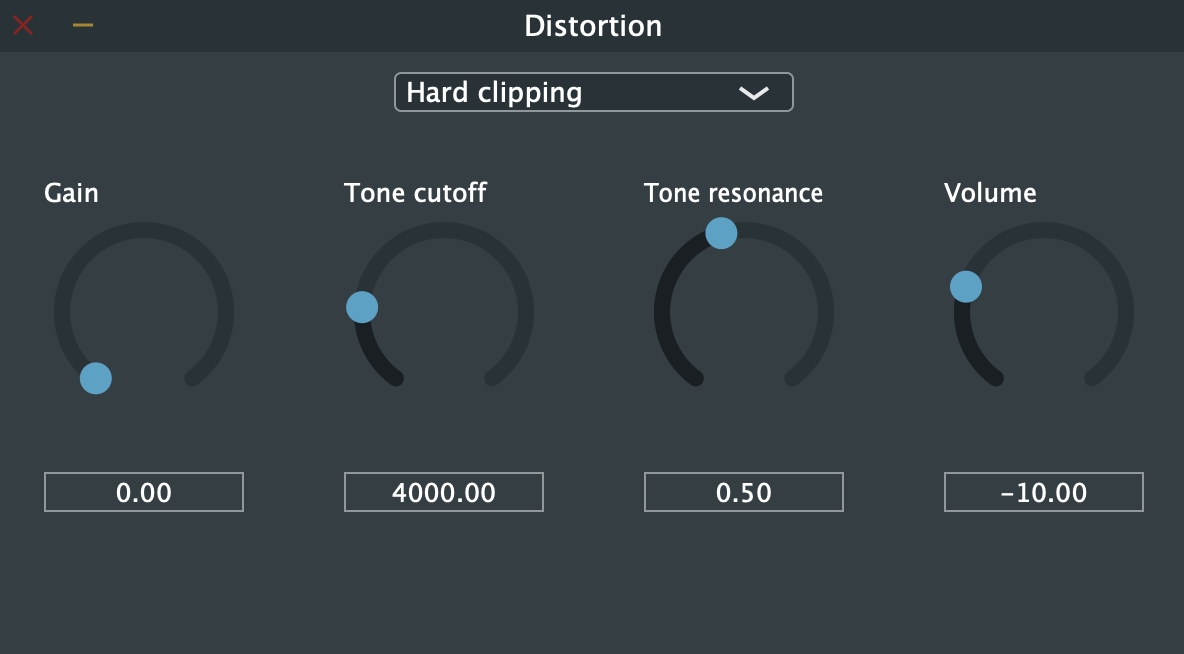
\includegraphics[scale=0.7]{gui.png}
		\centering
		\caption{Plugin's GUI}
		\label{fig:gui}
	\end{figure}

	Our plugin has been developed using a simple GUI, in Figure[\ref{fig:gui}], with the following graphic components:
	\\
	
	
	-	Gain knob 
	
	-	Tone cutoff knob 
	
	-	Tone resonance knob
	
	-	Volume knob
	
	-	Distortion type dropdown menu
	\\
	
	
	The gain knob is used to choose the level of the distortion effect applied to the sound, without affecting the output volume.
	
	The two tone knobs are used to control the brightness of the sound, changing the parameters of a IIR low pass filter applied as last step of the computation. In particular, with one knob we can control the cutoff frequency of the LPF and with the other we can control its resonance. 
	
	The volume knob allows the user to change the output amplitude of the sound.
	
	The dropdown menu is used to change the type of distortion effect applied to the sound. We have implemented five types of distortion: hard clipping, soft clipping exponential, soft clipping quadratic, full wave rectification and half wave rectification.
	
	\section{Implementation}
	
	Our distortion plugin has been developed in C++, as programming language, using the JUCE cross-platform framework. We have followed a standard JUCE audio plugin development, implementing the two main classes Audio Processor and Audio Processor Editor. 
	Using this standard structure, we have been able to divide the more graphical part, implemented in the Audio Processor Editor class, from the one dedicated to audio processing, developed in the Audio Processor class.
	\\
	
	\textbf{-	Audio Processor Editor} 
\\
	
	In this class we have designed the Graphic User Interface by adding to the plugin window the graphic components we have needed: rotary sliders, in order to design the gain, tone and volume knobs, and a combo box menu, in Figure[\ref{fig:combobox}], in order to design the dropdown menu with which the user can choose the type of distortion effect to introduce.
	
	After having defined them, we have given to each element a fixed position and a size using the setBounds method.
	We haven’t redrawn the style of the graphical elements with the LookAndFeel class but we have used the standard components.
	\\
	
	\begin{figure}[h!]
		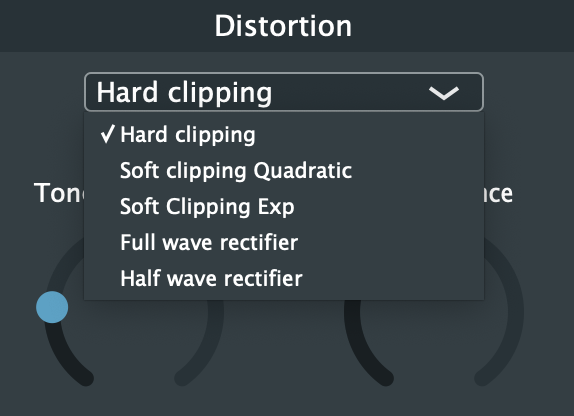
\includegraphics[scale=0.6]{combobox.png}
		\centering
		\caption{Dropdown menu}
		\label{fig:combobox}
	\end{figure}

	The connection between graphical elements and the Processor has been implemented using the AudioProcessorValueTreeState class. This method is an alternative to the Listener class, in order to connect each graphical component directly to a corresponding Audio Parameter.
	
	In particular, using  a SliderAttachment object for each Slider, we have maintained a connection between the graphical Slider element and a parameter in AudioProcessorValueTreeState, keeping the two things in sync. We have used the same approach with a ComboBoxAttachment object to maintain the dropdown menu state.
	\\
	
	\textbf{-	Audio Processor }\\
	
	The Audio Processor class contains the implementation of the distortion effect as well as the logic behind the different knobs.
	In the header file we defined some useful variables such as:
	\\
	
	-	oversampling: an object of class juce::dsp::Oversampling
	
	-	antiAliasingFilter: an IIR filter used in order to avoid aliasing after the oversampling
	
	-	toneFilter: an IIR tone-shaper filter
	
	-	lastSampleRate: sample rate of the input signal
	
	-	oversamplingFactor: the factor defining the oversampling step
	\\
	
	In the cpp file, specifically in the method processBlock, we followed the workflow in Figure[\ref{fig:workflow}].  As first step, we used the method processSamplesUp in order to perform the oversampling of the input signal.
	Then we implemented the logic for the different distortion effects simply by applying 5 different non-linear functions to the oversampled signal.
	After that we took the distorted signal and filtered it with an anti-aliasing low-pass filter with cut-off frequency equal to the original sampling rate divided by 2.
	Finally we downsampled the signal down to the original sampling rate and applied anotherlow-pass filter with the purpose of shaping the sound of the distorted signal.  
	
	\begin{figure}[h!]
		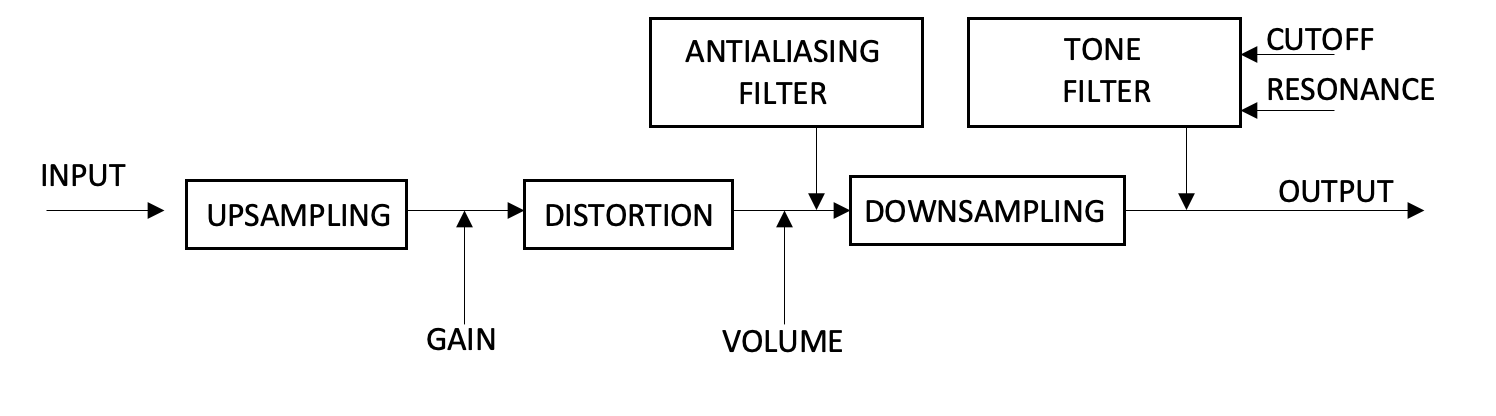
\includegraphics[scale=0.5]{workflow.png}
		\centering
		\caption{Plugin's workflow}
		\label{fig:workflow}
	\end{figure}

	\section{GitHub Repository}
	\url{https://github.com/ElisaCastelli/CMLS-HW2-Group11.git}
	
	\medskip
	
	\begin{thebibliography}{99}
		\bibitem{juce} 
		
		JUCE: Jules' Utility Class Extensions,
		\\
		\url{https://juce.com/} 
		
		\bibitem{clipping} 
		Wikipedia page about clipping, 
		\\
		\url{https://en.wikipedia.org/wiki/Clipping_(audio)}
		
		\bibitem{distortion} 
		Wikipedia page about distortion, 
		\\
		\url{https://en.wikipedia.org/wiki/Distortion_(music)}
		
		\bibitem{oversampling} 
		Oversampling In Distortion Effects (Science of Sound),
		\\
		\url{https://science-of-sound.net/2016/06/oversampling-distortion-effects/}
		
	\end{thebibliography}
	
	
\end{document}
